\documentclass[a4paper]{article}
\usepackage[margin=1in]{geometry}
\usepackage[utf8]{inputenc}
\usepackage[english]{babel}
%\usepackage{graphicx}
\usepackage{amssymb}
\usepackage{amsmath}
\usepackage{amsthm}
%\usepackage{listings} % Darstellen von Codebeispielen
\usepackage{titlesec}
%\usepackage{chngcntr}
\usepackage{mathtools}
\usepackage{algorithm}
\usepackage{algpseudocode}
\usepackage[normalem]{ulem}
%\usepackage{float}
%\usepackage{cite}
\counterwithin{figure}{section}
\newcommand{\sectionbreak}{\clearpage}
\usepackage[round]{natbib}
\usepackage{float}
\usepackage{svg}
\usepackage{fancyhdr}
\pagestyle{fancy}
\usepackage[hidelinks]{hyperref}

\mathtoolsset{showonlyrefs}

\DeclareMathOperator{\argmax}{argmax}
\DeclareMathOperator{\argmin}{argmin}
%\DeclareMathOperator{\next}{next}
\DeclareMathOperator{\prev}{prev}
\DeclareMathOperator{\on}{on}
\DeclareMathOperator{\off}{off}
\DeclareMathOperator{\idle}{idle}
\DeclareMathOperator{\act}{active}
\DeclareMathOperator{\costs}{costs}
\DeclareMathOperator{\adjacent}{adjacent}
\DeclareMathOperator{\neighboring}{neighboring}
\DeclareMathOperator{\true}{true}
\DeclareMathOperator{\false}{false}
\DeclareMathOperator{\ifop}{if}
\DeclareMathOperator{\elseop}{otherwise}
\DeclareMathOperator{\OPT}{OPT}


\newtheorem{theorem}{Theorem}
\newtheorem{lemma}[theorem]{Lemma}
\newtheorem{definition}[theorem]{Definition}
%\newtheorem*{remark}{Remark}


\title{Greedy Energy-Efficient Scheduling Algorithms for Processor Systems}
%\author{Gunther Bidlingmaier}
%\date{15.11.2020}

\begin{document}

\selectlanguage{english}
%\frontmatter{}
%\input{pages/acknowledgements}

%\maketitle
\begin{abstract}
  We study a particular scheduling setting in which a set of $n$ jobs with individual release times and deadlines has to be scheduled across $m$ homogeneous processors while minimizing the consumed energy.
  Idle processors can be turned off so as to save energy, while turning them on requires a fixed amount of energy.
  For the special case of a single processor, the greedy algorithm Left-to-Right guarantees an approximation factor of $2$.
  We generalize this simple greedy policy to the case of multiple processors and show that the energy costs are still bounded by $2 \OPT + P$.
  Our algorithm has a running time of $(n + m) \log(d^*) F$ where $d^*$ is the largest deadline and $F$ the costs of a maximum flow calculation for checking feasibility of an instance.
\end{abstract}

\tableofcontents

\section{Algorithm}
\begin{algorithm}[H]
\caption{Parallel Left-to-Right}\label{alg:RECLTR}
\begin{algorithmic}
  \State{} $m_t \gets m$
  \State{} $l_t \gets 0$
  \For{$k \gets m$ \textrm{to} $1$}
    \State{$t\gets0$}
    \While{$t < d^*$}
      \State{$t \gets $\Call{KeepIdle}{k, t}}
      \State{$t \gets $\Call{KeepActive}{k, t}}
    \EndWhile{}
  \EndFor{}

  \Function{KeepIdle}{k, t}
    \State{search for maximal $t' \geq t$ s.t.\
    exists feasible schedule with $m_{t''} = k-1 \forall t'' \in [t, t')$}
    \State{$m_{t''} \gets k - 1 \forall t'' \in [t, t')$}
    \State{\Return{$t'$}}
  \EndFunction{}
  \Function{KeepActive}{k, t}
    \State{search for maximal $t' \geq t$ s.t.\
    exists feasible schedule with $l'_{t''} = \max\{k, l_{t''}\}k-1 \forall t'' \in [t, t')$}
    \State{$m_{t''} \gets k - 1 \forall t'' \in [t, t')$}
    \State{\Return{$t'$}}
  \EndFunction{}
  %\Function{IsFeasible}{\null}
  %  \State{$f^* \gets$ Max-Flow for current values of $m_t, l_t$}
  %  \State{\Return{$f^* == P$}}
  %\EndFunction{}
\end{algorithmic}
\end{algorithm}


\begin{figure}[H]
  \centering
  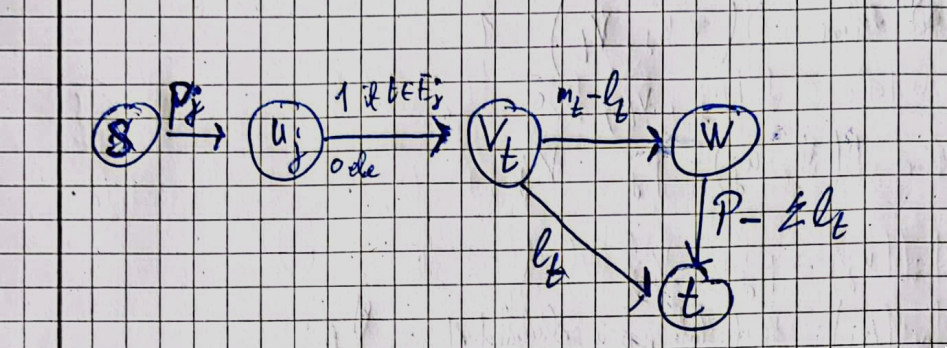
\includegraphics[width=\textwidth]{graphics/sketches/flow_network.png}
  \label{fig:flow}
  \caption{The Flow-Network for checking feasibility of a scheduling instance with lower and upper bounds $l_t$ and $m_t$ for the number of active processors at $t$.}
\end{figure}

\begin{lemma}\label{lemma:flow_feasibility}
  There exists a feasible solution to a scheduling instance with lower and upper bounds $l_t, m_t$ if and only if the maximum $s$-$t$ flow in the corresponding flow network depicted in Figure~\ref{fig:flow} has value $P$.
\end{lemma}
\begin{proof}
  Let $f$ be a $s$-$t$ flow of value $|f| = P$.
  We construct a feasbile schedule from $f$ respecting the lower and upper bounds given by $l_t$ and $m_t$.
  For every $j \in J$ and  $t \in [0, d^*]$, if $f(u_j, v_t) = 1$, then schedule $j$ at slot $t$.
  Since $|f| = P$ and the capacity $c(\{s\}, V \setminus \{s\}) = P$, we have $f_{in}(u_j) = p_j$ for every $j \in J$.
  Hence $f_{out}(u_j) = \sum_{t \in E_j} f_{in}(v_t) = p_j$.
  Hence every job $j$ is scheduled in $p_j$ distinct time slots.

  The schedule respects the upper bounds $m_t$, since $c(v_t, w) + c(v_t, t) \leq m_t - l_t + l_t$ and for every $t$ at most $m_t$ jobs are scheduled at $t$. 

  The schedule respects the lower bounds $l_t$, since
  $c(V \setminus \{t\}, \{t\}) = P$ and hence
  $f(v_t, t) = l_t$ for every slot $t$.
  By flow conservation we then have $f_{in}(v_t) \geq l_t$ which implies that at least $l_t$ jobs are scheduled at every slot $t$.

  For the other direction consider a feasible schedule respecting the lower and upper bounds $l_t, m_t$.
  We construct a flow $f$ of value $P$ and show that it is maximal.

  If $j$ is scheduled at slot $t$ and hence $t \in E_j$,
  define $f(u_j, v_t) = 1$, otherwise $f(u_j, v_t) = 0$.
  Define $f(s, u_j) = p_j$ for every $j \in J$.
  Hence we have $f_{in}(u_j) = p_j$
  and $f_{out}(u_j)$ must be  $p_j$ since this corresponds to the number of distinct time slots in which $j$ is scheduled.
  Define $f(v_t, t) = l_t$ for every slot $t$.
  Define $f(v_t, w) = f_{in}(v_t) - l_t$.
  We have $f(v_t, w) \leq m_t - l_t$ since $f_{in}(v_t)$ corresponds to the number of jobs scheduled at $t$, which is at most $m_t$.
  We also have $f_{out}(v_t) = f_{in}(v_t) - l_t + l_t = f_{in}(v_t)$.

  Define $f(w, t) = P - \sum_t l_t$.
  Then $f_{in}(w) = \sum_t f_{in}(v_t) - l_t
  = \sum_t |\{j \in J \mid j~\text{scheduled at}~t\}| - \sum_t l_t$.
  Since the schedule is feasible, this corresponds to
  $f_{in}(w) = P - \sum_t l_t = f_{out}(w)$.

\end{proof}


%\bibliographystyle{plain}
\bibliographystyle{abbrvnat}
\setcitestyle{authoryear,open={(},close={)}}
\bibliography{references}
\end{document}
